% Lecture Template for ME3050-001-002-Tristan Hill - Spring 2020
% Dynamics Modeling and Controls
% Time Response - Lecture 3

% I am finally converting my stuff to BEAMER

% Document settings

%\documentclass{beamer}                  % for presentation ?
\documentclass[handout]{beamer}  % for handout ?
\usepackage{beamerthemesplit}
\usepackage{amsmath}
\usepackage{listings}
\usepackage{multicol}

\beamertemplateballitem

\definecolor{TTUpurple}{rgb}{0.3098, 0.1607, 0.5176} % TTU Purple (primary)
\definecolor{TTUgold}{rgb}{1.0000, 0.8666, 0.0000} % TTU Gold (primary)

\setbeamercolor{palette primary}{bg=TTUpurple,fg=TTUgold}
\setbeamercolor{palette secondary}{bg=black,fg=TTUgold}
\setbeamercolor{palette tertiary}{bg=black,fg=TTUpurple}
\setbeamercolor{palette quaternary}{bg=TTUgold,fg=black}
\setbeamercolor{structure}{fg=TTUpurple} % itemize, enumerate, etc
\setbeamercolor{section in toc}{fg=TTUpurple} % TOC sections

%\usefonttheme{professionalfonts}

\newcommand{\LNUM}{4\hspace{2mm}} % Lecture Number 

\newcommand{\vspcc}{\vspace{6mm}\\ } 
\newcommand{\vspc}{\vspace{3mm}\\ } 
\newcommand{\hspc}{\hspace{5mm} } 

\newcommand{\Lagr}{\mathcal{L}} % lagrangian

\newcommand{\secondtitle}{Common Questions this Week}% second line of the title of this presentation , aka the topic of this lecture

\title{Time Response - Lecture \LNUM}
\author{ME3050 - Dynamics Modeling and Controls} % original formatting from Mike Renfro, September 21, 2004

\date{April 15, 2020}

\begin{document}

\lstset{language=MATLAB,basicstyle=\ttfamily\small,showstringspaces=false}

% Title page1 
\frame{\titlepage \center\textbf{\secondtitle}\vspcc}


% Section 0: Outline
\frame{

\large \textbf{Lecture \LNUM - \secondtitle} \vspc

 \begin{itemize}

	\item The Step Input\vspc % Section 1: The Step Input

	\item Obtaining the Response Equations in Problem 1\vspc        % Section 2
	
	\item Using the Error function and the Time Constant\vspc %Section 3

	\item Stability and the Roots\vspace{2mm} % Section 4

\end{itemize}

}


%Section 1: Forced Response of a Second Order Model % I think this section goes in the next lecture... 
\section{ The Step Input}

\frame{
\frametitle{The Step Input}

\large The {\bf step function} is a mathematical concept that represents an instant change. 

\begin{multicols}{2}
	
	\underline{Heavyside's Step Function}\vspc
	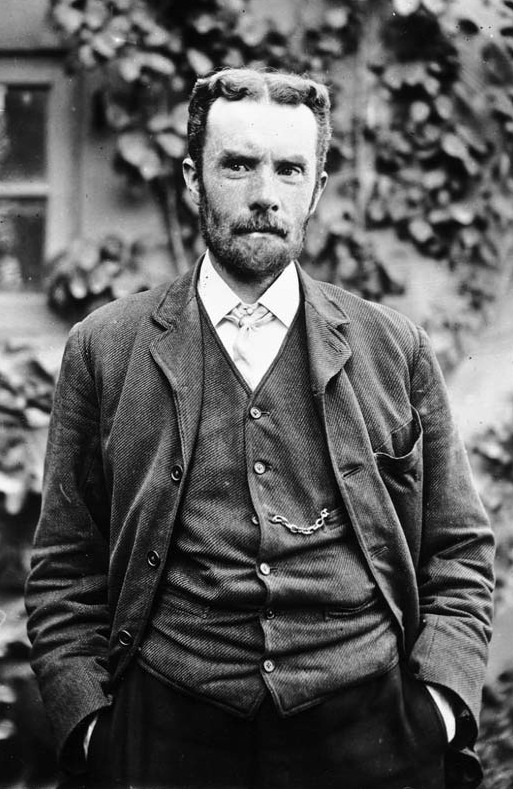
\includegraphics[scale=.1]{Oheaviside.jpg} \hspc  

	\[u_s(t) = \begin{cases} 
	      0 & t < 0 \\
	      1 & t\geq 0 \\
	   \end{cases}
	\]\\
	\[f_{step}(t) =Fu_s(t) 
		= \begin{cases} 
	      0 & t < 0 \\
	      F & t\geq 0 \\
	   \end{cases}
	\]\\

\end{multicols}


}



% section 2: Obtaining the Response Equations in Problem 1

\section{Obtaining the Response Equations in Problem 1}

\subsection{Obtaining the Response Equations in Problem 1}
\frame{
\frametitle{Obtaining the Response Equations in Problem 1}

You can see that each of the models in problem 1 is linear and first order. You do not have to re-derive (even though you easily could) the model but please reference where you found the equations you used. 



}

% section 3: Stability and the Roots

\section{Using the Error function and the Time Constant}

\subsection{Using the Error function and the Time Constant}
\frame{
\frametitle{Using the Error function and the Time Constant1}

}

% references is not a section for now, for looks and it would be a waste of space
\frame{

\frametitle{References}

\begin{itemize}
	\item System Dynamics, Palm III, Third Edition - Section 8.3 - Step Response of Second Order Systems
\end{itemize}

}
\end{document}









 